\chapter{Resolved atomization simulations of BIMER}
	\label{ch8:bimer_resolved_atomization}

Steps to follow (for this chapter):

\begin{enumerate}

	\item Intro: make it atractive. Specify that we are gonna simulate just one multipoint injector.
	
	\item Numerical setup: specify that :

		\begin{itemize}
		
			\item Fine mesh from the previous chapter is used
			
			\item One multipoint injector is going to be simulated (make zoom, nice pictures and graphs showing it)
			
			\item The simulation detailed in $\S$\ref{ch7:BIMER_application_point} is used as initial solution
			
			\item Describe the operating point ($q$, $We$). Mention how the bulk gas velocity has been obtained.
		
		\end{itemize}
	
\end{enumerate}

\newpage

\section{Introduction}

The multipoint burner BIMER was introduced in Chapter \ref{ch7:bimer_test_bench_and_aero}, where a study of the aerodynamic flow field for the operating conditions of interest was performed. Two operating points were simulated: the one tested by \citeColor[providakis_etude_2013] for which experimental data on the aerodynamic field was available, which was used for validating the simulations performed with YALES2; and the one tested by \citeColor[renaud_high-speed_2015] which provides experimental data on the non-reactive spray state. 

In this chapter, resolved simulations of the atomization process through one injector of the BIMER take-off stage, as done in Chapter \ref{ch5:jicf_resolved_simulations} for the academic JICF test case, are performed. The numerical setup and liquid injection operating point are described in $\S$\ref{sec:ch8_BIMER_computational_setup} and $\S$\ref{sec:ch8_BIMER_operating_condition} respectively. Then, the inlet velocity profiles from the aerodynamic computations which is seen by the atomizer is discussed in $\S$\textbf{XX}. Results from resolved atomization simulations performed for \textbf{XX} interface mesh resolutions are shown in $\S$\textbf{XX}. Finally, injectors learnt and built from such simulations are discussed in $\S$\textbf{XX}. These injectors are later used to initialise spray simulations at BIMER in Chapter \ref{ch9:BIMER_lagrangian}.



\section{Computational setup}
\label{sec:ch8_BIMER_computational_setup}

The computational geometry for performing the resolved atomization simulations is the same one as the one used for the aerodynamic ones, displayed in Figure \ref{fig:BIMER_geometry_full_domain}. The fine mesh from Figure \ref{fig:BIMER_mesh_fine} is used, its details provided in Table \ref{tab:BIMER_meshes_gaseous}. The aerodynamic field described in $\S$\ref{ch7:BIMER_application_point} is used as initial condition for the resolved atomization simulations. The boundary conditions are also the same ones in all the boundary except for the liquid injection point, which for the aerodynamic simulations it was specified as solid wall and for the resolved ones is changed to inlet. 

The location of the liquid injection point in the take-off stage is shown in Figure \ref{fig:BIMER_geometry_flower_details}. The injector consists of a nozzle with 8 mm length and a circular cross-section of diameter 0.3 mm. The injection nozzle can be appreciated in Figure \ref{fig:BIMER_liquid_injector_views}, where zoomed-in views of the liquid injection point rear and front sides are shown. The direction of the incoming air $u_g$ and the liquid injection $u_l$ are detailed, as well as the crossflow direction $x_c$ obtained from the resolved atomization simulations (see $\S$\ref{ch8:resolved_atomization_simulations}). A cut of the mesh in the injector is appreciated in the left figure: the cell size within the injector has been set to \textbf{XX} mm, and the walls are refined to \textbf{XX} mm. The right figure shows the dimensions of the gaseous inlet channel, which yield a hydraulic diameter of $D_h = 7.5$ mm. 


\begin{figure}[h!]
	\centering
	\includeinkscape[inkscapelatex=false,scale=0.2]{./part3_applications/figures_ch8_resolved/geometry_BIMER_liquid_injector_view/BIMER_liquid_injector_views_2}
	\caption[View of liquid injection point in BIMER]{View of liquid injection point in BIMER. The central figure shows the multipoint injector previously displayed in Figure \ref{fig:BIMER_geometry_flower_details}. The rectangular section shows zoomed-in views of the rear (\textsl{left}) and front (\textsl{right}) sides of the liquid injection point. The rear side shows the nozzle where the liquid inlet boundary condition is applied, and a view of the mesh within the injector. The front side (with transparency in the walls) the injection point where liquid is injected at velocity $u_l$, the crossflow direction $x_c$, and the gaseous inlet channel between two vanes of size 6 x 10 mm$^2$ where enters at a bulk velocity $u_g$.}%{View of liquid injection point in BIMER. The right top figure shows the injection nozzle. A zoomed view of the rectangular section is shown in the right bottom display, where a cut of mesh inside the injector is observed.}
	\label{fig:BIMER_liquid_injector_views}
\end{figure}

\subsection*{Sampling planes in BIMER}

The purpose of the BIMER resolved simulations is to characterize the produced spray in order to create lagrangian injectors with the SLI methodology to initialize dispersed phase computations. Therefore, the spray must be sampled in the fashion as it was done for the DLR JICF, whose sampling planes were shown in Figure \ref{fig:jicf_interior_boundaries_surface_measurements}. In that test case, the defined sampling planes were perpendicular to the crossflow axis $x$, since the jet deviates and atomizes producing a spray that moves in this direction. BIMER presents a more complex geometry representative of real injection systems where the absolute reference system is not aligned with the liquid fuel injection point chosen. Therefore, it is convenient to change the reference system to a local one which is aligned with the jet deviation direction (i.e. the local crossflow direction). This direction is denoted as $x_c$ and is shown in Figure \ref{fig:BIMER_liquid_injector_views} right. It has been obtained by performing resolved simulations and checking visually the JICF direction. The local reference system is defined by the orthogonal coordinates $\left( x_c, y_c, z_c \right)$ obtained through a transformation from the global coordinate system. This local system, shown in Figure \ref{fig:BIMER_local_FoR_and_sampling_planes}, is centered at the liquid injection point. The figure also shows the location of the sampling planes, which are perpendicular to the $x_c$ axis and are expressed in relation to the injection diameter $d_\mathrm{inj}$.

\begin{figure}[h!]
	\centering
	\includeinkscape[inkscapelatex=true,scale=0.8]{./part3_applications/figures_ch8_resolved/BIMER_local_FoR_and_sampling_planes}
	\vspace*{-0.5in}
	\caption{Instaneous snapshot of liquid injection in BIMER shown the local coordinate system and the location of spray sampling planes. \textbf{XX OJO: actualizar con sampling planes finales.}}
	\label{fig:BIMER_local_FoR_and_sampling_planes}
\end{figure}


\section{Operating condition}
\label{sec:ch8_BIMER_operating_condition}

The ambient conditions and inlet gaseous flow rate for the operating point to study are shown in Table \ref{tab:gaseous_operating_points_BIMER}. These ones characterize the aerodynamic field of the overall burner. To determine now the operating point and classify it into the JICF breakup map, the liquid and gaseous parameters relevant to the single multipoint injector need to be stated.

%\begin{equation}
%x/d_\mathrm{inj} ~~ ; ~~ \textcolor{blue}{z/d_\mathrm{inj} }
%\end{equation}

\subsection{Gaseous phase}

According to \citeColor[barbosa_etude_2008], $80 \%$ of the air flow rate goes through the take-off stage and $20 \%$ goes through the take-off one. The study of \citeColor[renaud_high-speed_2015] shows that the percentage through the pilot is actually $13.5 \%$, hence $86.5 \%$ goes through the take-off. Considering the application point in Table \ref{tab:gaseous_operating_points_BIMER}, this makes a total of $\dot{m}_{g,\mathrm{takeoff}} = 37.2815 ~ $ g s$^{-1}$, which corresponds to a flow rate $Q = 0.04567 $ m$^{3}$ s$^{-1}$. Since that this flow rate is split through 20 vanes, the flow rate per canal is $Q_g = 2.2833 \cdot 10^{-3}$ m$^{3}$ s$^{-1}$. With an area of 6x10 mm$^2$ (see Figure \ref{fig:BIMER_liquid_injector_views}), the estimated gas bulk velocity is:

\begin{equation}
u_g = Q_g/A = 38 ~ \mathrm{m} ~ \mathrm{s}^{-1}
\end{equation}

\subsection{Liquid phase}

In the operating point studied, the total liquid mass flow rate injected is $\dot{m}_{l,\mathrm{total}} = 1.64$ g s$^{-1}$. The staging parameter, defined in Eq. (\ref{eq:BIMER_staging_parameter}), is $\alpha = 15 ~\%$, meaning that amount of liquid goes through the pilot stage and $85 ~\%$ of fuel goes through the take-off. Therefore, $\dot{m}_{l,\mathrm{pilot}} = 0.25$ g s$^{-1}$ and $\dot{m}_{l,\mathrm{takeoff}} = 1.39$ g s$^{-1}$. This quantity of fuel is injected through 10 injection holes that conform the take-off stage; assuming that fuel repartition is done equally through all the channels, each injector introduces $0.139$ g s$^{-1}$ of dodecane fuel, which is equivalent to a flow rate of $Q_l = 185.3$  mm$^3$ s$^{-1}$ given the dodecane density from Table \ref{tab:dodecane_properties}. From this flow rate, the bulk liquid velocity $u_l$ can be estimated knowing an injection diameter of $d_\mathrm{inj} = 0.3$ mm:

\begin{equation}
u_l = \frac{Q_l}{\pi d_\mathrm{inj}^2 / 4} = 2.6 ~ \mathrm{m} ~ \mathrm{s}^{-1}
\end{equation}


The velocity profile imposed at the liquid inlet shown in Figure \ref{fig:BIMER_liquid_injector_views} \hl{is a Poiseuille profile with the mean velocity of value $u_l$}. With the estimate values for bulk liquid and gaseous velocities, the liquid properties given in Table \ref{tab:dodecane_properties} and the gaseous properties from Table \ref{tab:gaseous_operating_points_BIMER}, the momentum flux ratio $q$ and the Weber number based on the gaseous phase $We_g$ can now be calculated:

%\begin{subequations}
%\begin{align}
%q &=  \frac{\rho_l u_l^2}{\rho_g u_g^2} \approx 4 \\
%We_g &=  \frac{\rho_g d_{inj} u_g^2}{\sigma} \approx 14
%\end{align}
%\end{subequations}

\begin{equation}
q =  \frac{\rho_l u_l^2}{\rho_g u_g^2} \approx 4 ~~~~ ; ~~~~  We_g =  \frac{\rho_g d_\mathrm{inj} u_g^2}{\sigma} \approx 14
\end{equation}

%\begin{subequations}
%\begin{align}
%q &=  \frac{\rho_l u_l^2}{\rho_g u_g^2} = \frac{750 \cdot 2.6^2}{0.816382 \cdot 38.05^2} = 4 \\
%We_g &=  \frac{\rho_g d_{inj} u_g^2}{\sigma} = \frac{0.816382 \cdot 0.3 mm \cdot 38.05^2}{25.35 10^{-3}} \approx 14
%\end{align}
%\end{subequations}

Figure \ref{fig:location_BIMER_op_in_breakup_map} shows the BIMER JICF operating point classified in the breakup diagram of \citeColor[wu_breakup_1997]. As observed, in this case the breakup regime corresponds to bag breakup.

The governing parameters characterizing the BIMER operating point are summarized in Table \ref{tab:bimer_sps_operating_point}. The dimensionless numbers from Eqs. (\ref{eq:dimensionless_numbers_jicf}) are also calculated. Two simulations have been performed with two values for the interface mesh size $\Delta x_\mathrm{min}$, the nomenclature for each case is given in Table \ref{tab:BIMER_resolved_simulations_performed}.


\begin{table}[!h]
\centering
\caption{BIMER operating point to perform resolved atomization simulations}
\begin{tabular}{lccc}
\thickhline
\textbf{Parameter} & \textbf{Symbol} & \textbf{Units} &  \textbf{Value} \\
\thickhline
Nozzle diameter & $d_\mathrm{inj}$ & mm & 0.3 \\
%\hline
Gas bulk velocity & $u_g$ & m s$^{-1}$ & 38 \\
%\hline
Gas flow rate & $Q_g$ & m$^3$ s$^{-1}$ & $2.2833 \cdot 10^{-3}$   \\
%\hline
Liquid bulk velocity & $u_l$ & m s$^{-1}$ & 2.6  \\
%\hline
Liquid flow rate & $Q_l$ & mm$^3$ s$^{-1}$ & 185.3  \\
%\hline
Ambient pressure & $p_\mathrm{amb}$ & bar &  1 \\
%\hline
Gas temperature & $T_g$ & K & 433 \\
%\hline
Liquid temperature & $T_l$ & K &  \\
%\hline
Gas density & $\rho_g$ & kg m$^{-3}$ & 0.82 \\
%\hline
Liquid density & $\rho_l$ & kg m$^{-3}$ & 750 \\
%\hline
Gas viscosity & $\mu_g$ & kg m$^{-1}$ s$^{-1}$ & $2.39 \cdot 10^{-5}$ \\
%\hline
Liquid viscosity & $\mu_l$ & kg m$^{-1}$ s$^{-1}$ &  $1.36 \cdot 10^{-3}$ \\
%\hline
Surface tension & $\sigma$ & kg s$^{-2}$ &  0.025  \\
\thickhline
Gas Reynolds number & $Re_g$ & - & $9.80 \cdot 10^3$ \\
%\hline
Liquid Reynolds number & $Re_l$ & - & 430 \\
%\hline
Momentum ratio & $q$ & - & 4  \\
%\hline
Gas Weber number & $We_g$ & - & 14 \\
%\hline
Liquid Weber number & $We_l$ & - & 60 \\
%\hline
Relative Weber number & $We_\mathrm{rel}$ & - & 12 \\
%\hline
Aerodynamic Weber number & $We_\mathrm{aero}$ & - & 0.067 \\
%\hline
Ohnesorge number & $Oh $ & - & 0.018 \\
%\hline
Density ratio & $r$ & - & 915 \\
%\hline
\thickhline
\end{tabular}
\label{tab:bimer_sps_operating_point}
\end{table}

\begin{table}[!h]
\centering
\caption{Nomenclature for resolved atomization simulations}
\begin{tabular}{cc}
\thickhline
%$\pmb{\Delta} x_\mathrm{min}$ [$\pmb{\mu}$$\textbf{m}])  &  \multicolumn{2}{c}{\textbf{Operating condition}} \\ 
$\Delta x_\mathrm{min}$ [$\mu$m]  &  Denomination \\ 
\thickhline
7.5 & BIMER\_DX07 \\
10 & BIMER\_DX10 \\
15 & BIMER\_DX15 \\
\thickhline
\end{tabular}
\label{tab:BIMER_resolved_simulations_performed}
\end{table}


\clearpage

\begin{figure}[ht]
     \centering
     \includeinkscape[inkscapelatex=false,scale=0.45]{./part3_applications/figures_ch8_resolved/BIMER_breakup_regime_our_operating_point}
     \vspace*{-0.2in}
     \caption{Location of simulated operating condition in the breakup map by \citeColor[wu_breakup_1997]}
	% See: https://stackoverflow.com/questions/35210337/can-i-plot-several-histograms-in-3d/35225919
      \label{fig:location_BIMER_op_in_breakup_map}
\end{figure}



\section{Initial conditions}

The aerodynamic field inside BIMER for the operating points of interest was discussed in Chapter \ref{ch7:bimer_test_bench_and_aero}. From this study, a fine mesh consisting of 38 million elements was chosen (see Table \ref{tab:BIMER_meshes_gaseous}). The gaseous field for the application point, which is the chosen one to perform spray simulations, was studied in $\S$\ref{ch7:BIMER_application_point}. This solution is taken as the initial condition from the resolved atomization simulations. The mean and RMS velocity fields can be seen in Figure \ref{fig:field_application}. 


\section{Definition of liquid characteristic times}

Characteristic times can be defined for the liquid phase in BIMER in the same way it was done for the DLR JICF test case from Chapter \ref{ch5:jicf_resolved_simulations}. Details on the timescales chosen and on their calculation are given in $\S$\ref{sec:ch5_liquid_characteristic_times}. Here, the definitions summarized in Table \ref{tab:jicf_characteristic times} are directly applied to the BIMER test case. The results are shown in Table \ref{tab:BIMER_SPS_characteristic times}. 

\begin{table}[!h]
\centering
\caption{Characteristic physical timescales [$\mu$s] in BIMER simulations}
\begin{tabular}{ccc}
\thickhline
\textbf{Time scale} & \textbf{Expression} & \textbf{BIMER} \\
\thickhline
Inertia & $\tau_\mathrm{in} = \frac{d_\mathrm{inj}}{u_l}$ & 115.38 \\
Aerodynamic breakup  &  $\tau_\mathrm{ab} =  \frac{d_\mathrm{inj}}{u_g - u_l} \sqrt{\frac{\rho_l}{\rho_g}} $ & 256.30 \\
Non-aerodynamic breakup  &  $\tau_\mathrm{nb} = \frac{d_\mathrm{inj}}{u_l} We_l^{1/3} $ &  453.81 \\
Capillary & $\tau_\mathrm{cap} = \sqrt{\frac{\rho_l d_\mathrm{inj}^3}{8 \sigma}}$ & 318.20 \\
\thickhline
\end{tabular}
\label{tab:BIMER_SPS_characteristic times}
\end{table} 

As shown in the previous table, the lower timescale is found for the inertia processes and hence those are governing breakup. Yet, all timescales are of the same order of magnitude, as opposed to the timescales of the DLR JICF summarized in Figure \ref{tab:jicf_characteristic times} where the fastest timescale (inertia) was around $100$ times smaller than the slowest (capillary). For the BIMER operating point studied, the inertia timescale is only $3$ times smaller than the capillary one, which is not even the slowest (in this case, it corresponds to the non-aerodynamic breakup timescale). The fact that the timescales in this case are closer to each other agree with the location of the BIMER operating point in the breakup diagram of Figure \ref{fig:location_BIMER_op_in_breakup_map} \citepColor[pilch_use_1987]. Besides the physical timescales, the droplets arrival times to the sampling planes depicted in Figure \ref{fig:BIMER_local_FoR_and_sampling_planes}. These ones are summarized in Table \ref{BIMER_SPS_characteristic_droplet_sampling_times}. 

\clearpage

\begin{table}[!h]
\centering
\caption{Characteristic droplet arrival times to sampling planes $\tau_\mathrm{dr_{x_c}}$ [$\mu$s] in BIMER simulations}
\begin{tabular}{ccccc}
\thickhline
\textbf{Case} & $x_c/d_\mathrm{inj} = 5$ & $x_c/d_\mathrm{inj} = 10$ & $x_c/d_\mathrm{inj} = 15$ \\
\thickhline 
BIMER\_DX07 & - & - & -  \\
BIMER\_DX10 & - & - & -  \\
BIMER\_DX15  & - & - & - \\
\thickhline
\end{tabular}
\label{tab:BIMER_SPS_characteristic_droplet_sampling_times}
\end{table}






\section{Jet evolution}

In first place, the jet evolution at the early instants of the injection process is shown in Figure \ref {fig:BIMER_jet_establishment}. As in the simulations from Chapter \ref{ch5:jicf_resolved_simulations}, snapshots are shown for values of dimensionless time $t^*$ defined by Eq. (\ref{eq:t_dimensionless_with_tau_in}), in which the physical time is expressed in relation to the timescale $\tau_\mathrm{in}$ from Table \ref{tab:BIMER_SPS_characteristic times}. 



%\label{ch8:resolved_atomization_simulations}

%\begin{table}[!h]
%\centering
%\caption{Operating point}
%\begin{tabular}{cccc}
%\thickhline
%$u_g$ [m s$^{-1}$] &  38 \\
%\hline
%$u_l$ [m s$^{-1}$] &  2.6 \\
%\hline
%\hline
%$q$ & 4 \\ %4.3 \\
%\hline
%$We_g$ & 14 \\
%\hline
%\end{tabular}
%\label{tab:bimer_sps_operating_point}
%\end{table}
%
%\begin{table}[!h]
%\centering
%\caption{Operating point}
%\begin{tabular}{cccc}
%\thickhline
%$u_g$ [m s$^{-1}$] &  $u_l$ [m s$^{-1}$] & $q$ &  $We_g$  \\
%\hline
%38 &  2.6 & 4 & 15 \\
%\thickhline
%\end{tabular}
%\label{tab:bimer_sps_operating_point}
%\end{table}



%\begin{figure}[h!]	
%	\centering
%	\includeinkscape[inkscapelatex=false,scale=0.75]{./part1_numerical_approaches/figures_ch3/gas_injection_area_multipoint}
%	\caption{Area to calculate bulk gas velocity}
%	\label{fig:gas_injection_area_multipoint}
%\end{figure}


%According to \textbf{2016 Eckel}, the velocity is not the gaseous one but the relative:
%
%\begin{equation}
%\tau_c = \sqrt{\frac{\rho_l}{\rho_g}} \frac{d_\mathrm{inj}}{u_\mathrm{rel}} = \sqrt{\frac{750}{0.816382 }} \frac{0.3 ~mm}{38 - 2.6} = 0.26
%\end{equation}
%
%which is actually very similar.

\begin{figure}[ht]
\centering
\includeinkscape[inkscapelatex=false,scale=0.7]{./part3_applications/figures_ch8_resolved/jet_evolution}
\caption[Establishment of BIMER resolved atomization simulations at several time instants.]{Establishment of BIMER resolved atomization simulations at several time instants. \textsl{Left}: DX07. \textsl{Center}: DX10. \textsl{Right}: DX15. }
\label{fig:BIMER_jet_establishment}
\end{figure}

\subsection{Breakup topology}

The topology is super different with respecto to DLR JICF!! 

\subsection{Jet establishment}

Figure \ref{fig:BIMER_volume_nelem_evolution} shows the evolution of liquid volume and of mesh size for the three simulations performed. 

\begin{figure}[ht]
\flushleft
\begin{subfigure}[b]{0.45\textwidth}
	\centering
   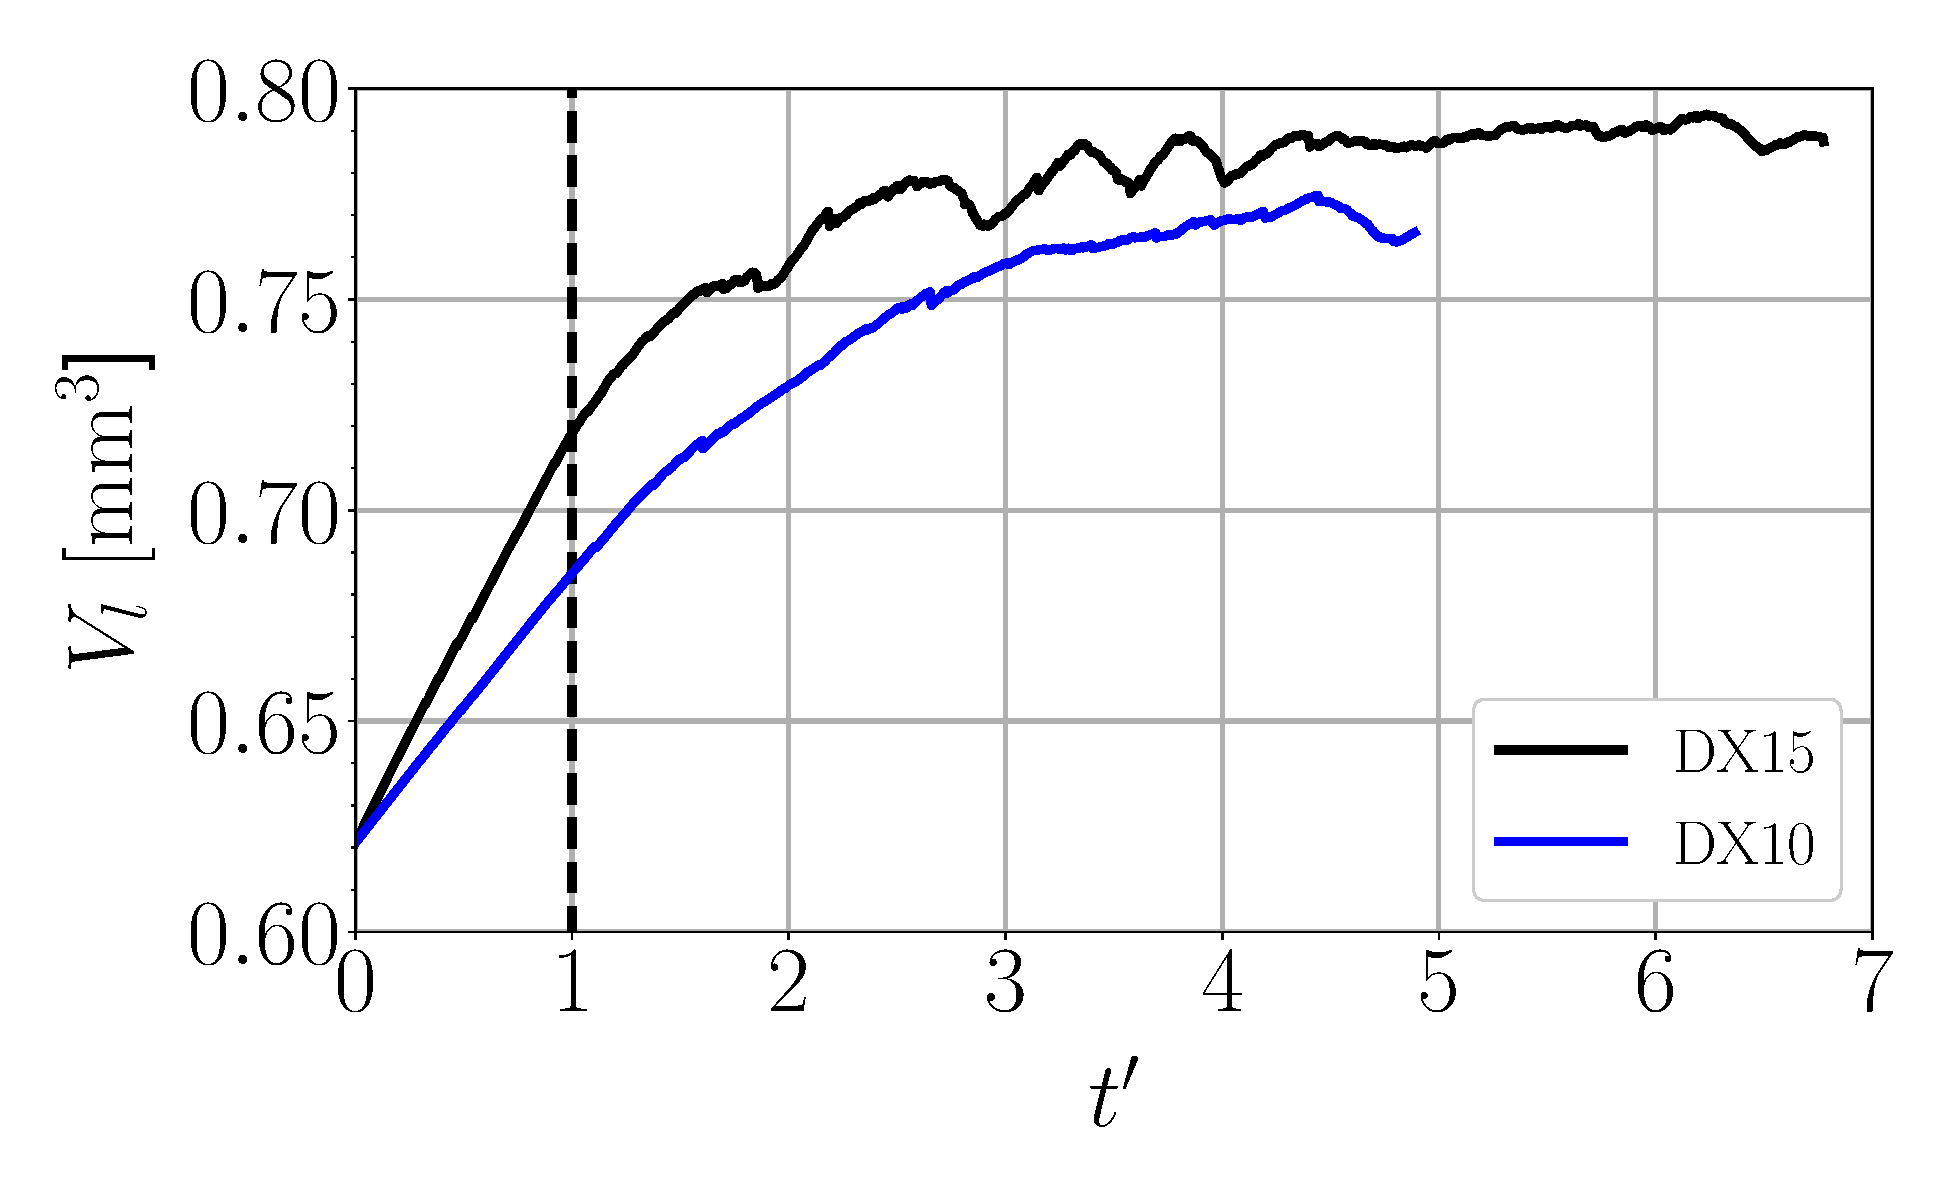
\includegraphics[scale=0.24]{./part3_applications/figures_ch8_resolved/BIMER_liquid_volume_increase}
   %\caption{Liquid volume}
   \label{fig:BIMER_liquid_volume_evolution} 
\end{subfigure}
\hfill
\begin{subfigure}[b]{0.45\textwidth}
	\centering
   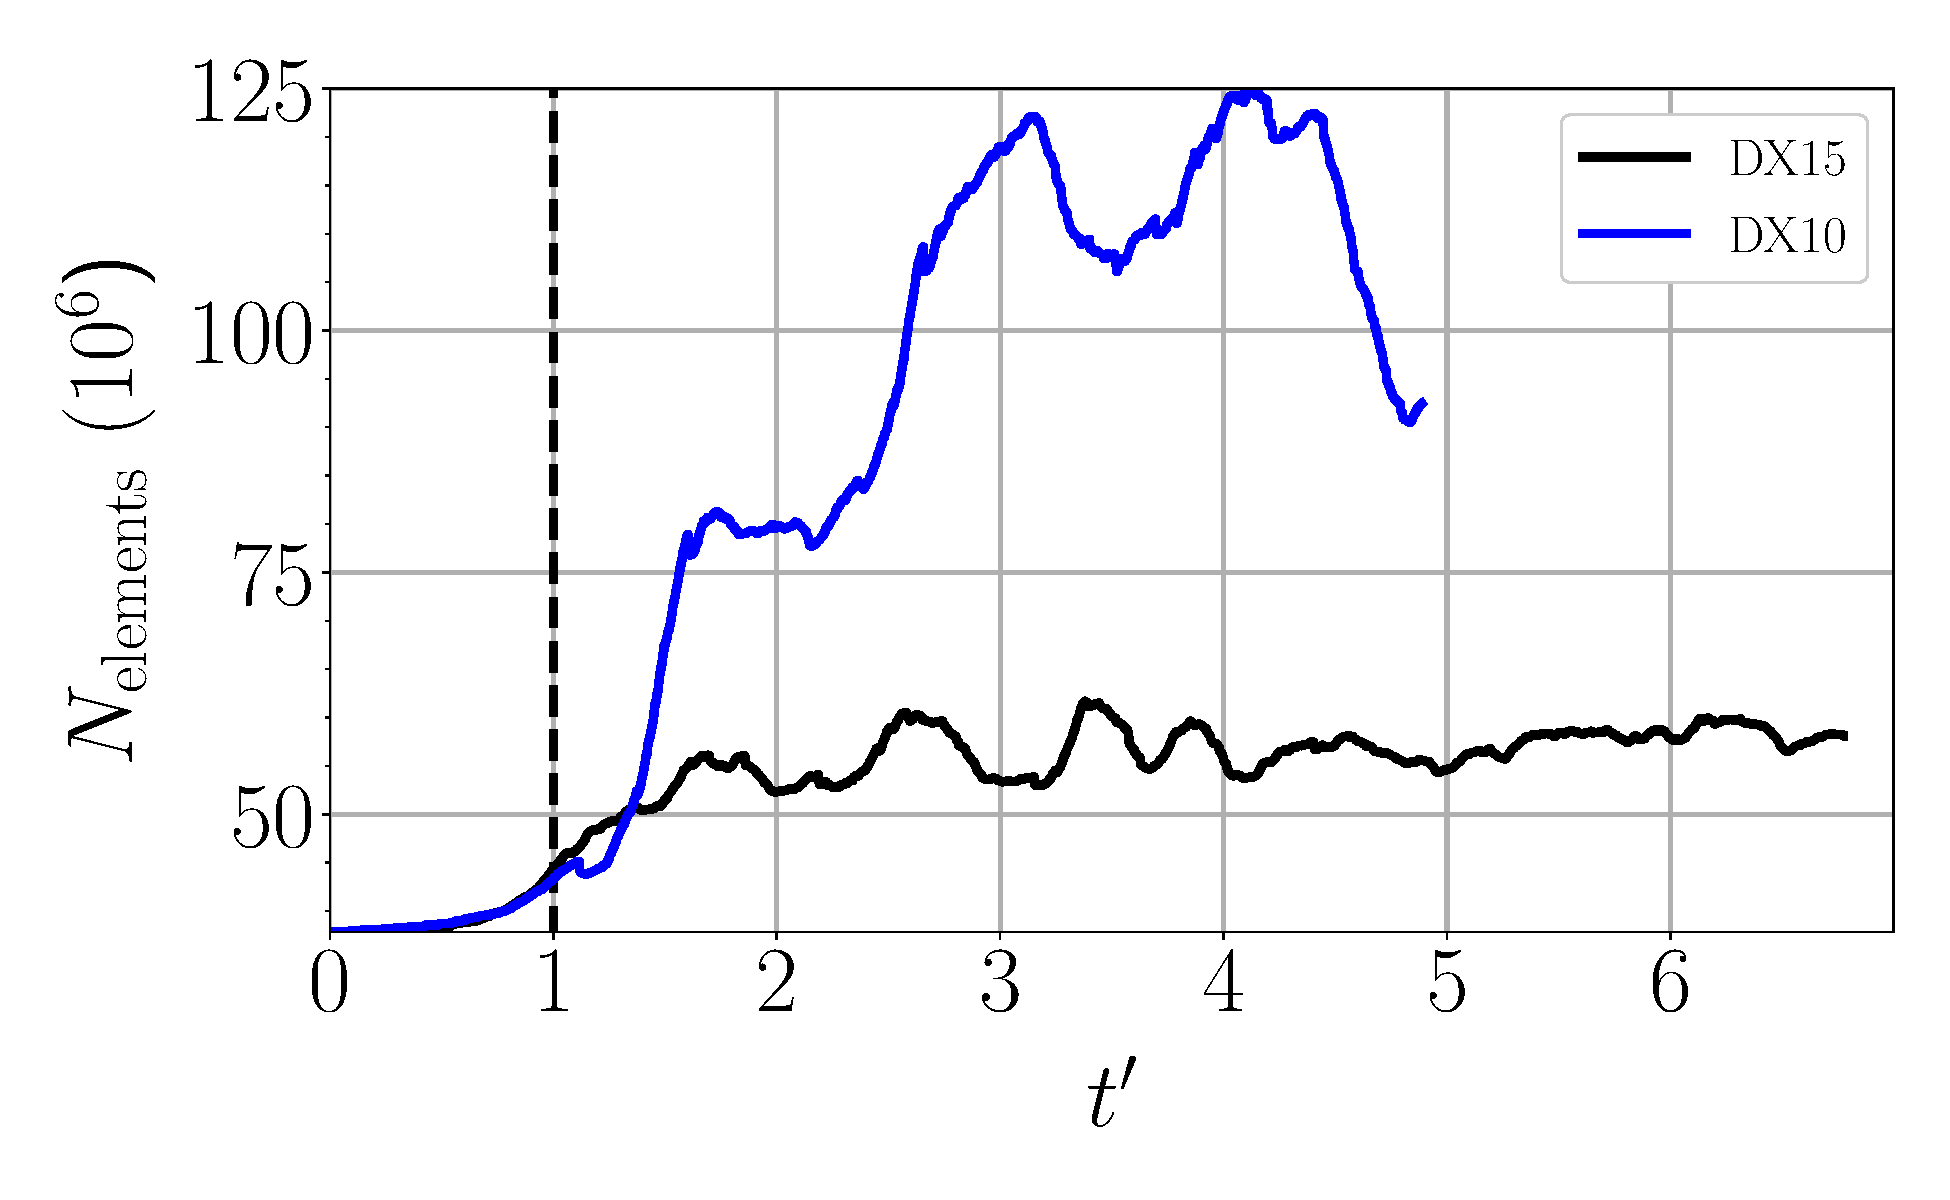
\includegraphics[scale=0.24]{./part3_applications/figures_ch8_resolved/BIMER_nelem_increase}
   %\caption{Zoomed-in view of Figure \ref{fig:JICF_nelem_increase_all_t} in range $t^{\prime} \in [0, 2]$}
   \label{fig:BIMER_nelem_increase}
\end{subfigure}
   \caption{Evolution of number of mesh elements (\textsl{left}) and number of mesh elements (\textsl{right}) with time in BIMER resolved simulations.}
\label{fig:BIMER_volume_nelem_evolution}
\end{figure}


\section{Dense core characterization}
%\label{ch8:resolved_atomization_simulations}





\section{Direct measurement of liquid fluxes}



\section{Spray characterization}

\section{Smart Lagrangian Injectors}
\label{sec:ch8_learning_SLI_in_BIMER}



\section{Computational performances}


\section{Learning injectors}




\section{Conclusion}
